\documentclass{llncs}
\usepackage{hyperref}
\usepackage{url}
\pagestyle{plain}
\usepackage{threeparttable}
%%%%% NEW MATH DEFINITIONS %%%%%

\usepackage{amsmath,amsfonts,bm}

% Mark sections of captions for referring to divisions of figures
\newcommand{\figleft}{{\em (Left)}}
\newcommand{\figcenter}{{\em (Center)}}
\newcommand{\figright}{{\em (Right)}}
\newcommand{\figtop}{{\em (Top)}}
\newcommand{\figbottom}{{\em (Bottom)}}
\newcommand{\captiona}{{\em (a)}}
\newcommand{\captionb}{{\em (b)}}
\newcommand{\captionc}{{\em (c)}}
\newcommand{\captiond}{{\em (d)}}

% Highlight a newly defined term
\newcommand{\newterm}[1]{{\bf #1}}


% Figure reference, lower-case.
\def\figref#1{figure~\ref{#1}}
% Figure reference, capital. For start of sentence
\def\Figref#1{Figure~\ref{#1}}
\def\twofigref#1#2{figures \ref{#1} and \ref{#2}}
\def\quadfigref#1#2#3#4{figures \ref{#1}, \ref{#2}, \ref{#3} and \ref{#4}}
% Section reference, lower-case.
\def\secref#1{section~\ref{#1}}
% Section reference, capital.
\def\Secref#1{Section~\ref{#1}}
% Reference to two sections.
\def\twosecrefs#1#2{sections \ref{#1} and \ref{#2}}
% Reference to three sections.
\def\secrefs#1#2#3{sections \ref{#1}, \ref{#2} and \ref{#3}}
% Reference to an equation, lower-case.
\def\eqref#1{equation~\ref{#1}}
% Reference to an equation, upper case
\def\Eqref#1{Equation~\ref{#1}}
% A raw reference to an equation---avoid using if possible
\def\plaineqref#1{\ref{#1}}
% Reference to a chapter, lower-case.
\def\chapref#1{chapter~\ref{#1}}
% Reference to an equation, upper case.
\def\Chapref#1{Chapter~\ref{#1}}
% Reference to a range of chapters
\def\rangechapref#1#2{chapters\ref{#1}--\ref{#2}}
% Reference to an algorithm, lower-case.
\def\algref#1{algorithm~\ref{#1}}
% Reference to an algorithm, upper case.
\def\Algref#1{Algorithm~\ref{#1}}
\def\twoalgref#1#2{algorithms \ref{#1} and \ref{#2}}
\def\Twoalgref#1#2{Algorithms \ref{#1} and \ref{#2}}
% Reference to a part, lower case
\def\partref#1{part~\ref{#1}}
% Reference to a part, upper case
\def\Partref#1{Part~\ref{#1}}
\def\twopartref#1#2{parts \ref{#1} and \ref{#2}}

\def\ceil#1{\lceil #1 \rceil}
\def\floor#1{\lfloor #1 \rfloor}
\def\1{\bm{1}}
\newcommand{\train}{\mathcal{D}}
\newcommand{\valid}{\mathcal{D_{\mathrm{valid}}}}
\newcommand{\test}{\mathcal{D_{\mathrm{test}}}}

\def\eps{{\epsilon}}


% Random variables
\def\reta{{\textnormal{$\eta$}}}
\def\ra{{\textnormal{a}}}
\def\rb{{\textnormal{b}}}
\def\rc{{\textnormal{c}}}
\def\rd{{\textnormal{d}}}
\def\re{{\textnormal{e}}}
\def\rf{{\textnormal{f}}}
\def\rg{{\textnormal{g}}}
\def\rh{{\textnormal{h}}}
\def\ri{{\textnormal{i}}}
\def\rj{{\textnormal{j}}}
\def\rk{{\textnormal{k}}}
\def\rl{{\textnormal{l}}}
% rm is already a command, just don't name any random variables m
\def\rn{{\textnormal{n}}}
\def\ro{{\textnormal{o}}}
\def\rp{{\textnormal{p}}}
\def\rq{{\textnormal{q}}}
\def\rr{{\textnormal{r}}}
\def\rs{{\textnormal{s}}}
\def\rt{{\textnormal{t}}}
\def\ru{{\textnormal{u}}}
\def\rv{{\textnormal{v}}}
\def\rw{{\textnormal{w}}}
\def\rx{{\textnormal{x}}}
\def\ry{{\textnormal{y}}}
\def\rz{{\textnormal{z}}}

% Random vectors
\def\rvepsilon{{\mathbf{\epsilon}}}
\def\rvtheta{{\mathbf{\theta}}}
\def\rva{{\mathbf{a}}}
\def\rvb{{\mathbf{b}}}
\def\rvc{{\mathbf{c}}}
\def\rvd{{\mathbf{d}}}
\def\rve{{\mathbf{e}}}
\def\rvf{{\mathbf{f}}}
\def\rvg{{\mathbf{g}}}
\def\rvh{{\mathbf{h}}}
\def\rvu{{\mathbf{i}}}
\def\rvj{{\mathbf{j}}}
\def\rvk{{\mathbf{k}}}
\def\rvl{{\mathbf{l}}}
\def\rvm{{\mathbf{m}}}
\def\rvn{{\mathbf{n}}}
\def\rvo{{\mathbf{o}}}
\def\rvp{{\mathbf{p}}}
\def\rvq{{\mathbf{q}}}
\def\rvr{{\mathbf{r}}}
\def\rvs{{\mathbf{s}}}
\def\rvt{{\mathbf{t}}}
\def\rvu{{\mathbf{u}}}
\def\rvv{{\mathbf{v}}}
\def\rvw{{\mathbf{w}}}
\def\rvx{{\mathbf{x}}}
\def\rvy{{\mathbf{y}}}
\def\rvz{{\mathbf{z}}}

% Elements of random vectors
\def\erva{{\textnormal{a}}}
\def\ervb{{\textnormal{b}}}
\def\ervc{{\textnormal{c}}}
\def\ervd{{\textnormal{d}}}
\def\erve{{\textnormal{e}}}
\def\ervf{{\textnormal{f}}}
\def\ervg{{\textnormal{g}}}
\def\ervh{{\textnormal{h}}}
\def\ervi{{\textnormal{i}}}
\def\ervj{{\textnormal{j}}}
\def\ervk{{\textnormal{k}}}
\def\ervl{{\textnormal{l}}}
\def\ervm{{\textnormal{m}}}
\def\ervn{{\textnormal{n}}}
\def\ervo{{\textnormal{o}}}
\def\ervp{{\textnormal{p}}}
\def\ervq{{\textnormal{q}}}
\def\ervr{{\textnormal{r}}}
\def\ervs{{\textnormal{s}}}
\def\ervt{{\textnormal{t}}}
\def\ervu{{\textnormal{u}}}
\def\ervv{{\textnormal{v}}}
\def\ervw{{\textnormal{w}}}
\def\ervx{{\textnormal{x}}}
\def\ervy{{\textnormal{y}}}
\def\ervz{{\textnormal{z}}}

% Random matrices
\def\rmA{{\mathbf{A}}}
\def\rmB{{\mathbf{B}}}
\def\rmC{{\mathbf{C}}}
\def\rmD{{\mathbf{D}}}
\def\rmE{{\mathbf{E}}}
\def\rmF{{\mathbf{F}}}
\def\rmG{{\mathbf{G}}}
\def\rmH{{\mathbf{H}}}
\def\rmI{{\mathbf{I}}}
\def\rmJ{{\mathbf{J}}}
\def\rmK{{\mathbf{K}}}
\def\rmL{{\mathbf{L}}}
\def\rmM{{\mathbf{M}}}
\def\rmN{{\mathbf{N}}}
\def\rmO{{\mathbf{O}}}
\def\rmP{{\mathbf{P}}}
\def\rmQ{{\mathbf{Q}}}
\def\rmR{{\mathbf{R}}}
\def\rmS{{\mathbf{S}}}
\def\rmT{{\mathbf{T}}}
\def\rmU{{\mathbf{U}}}
\def\rmV{{\mathbf{V}}}
\def\rmW{{\mathbf{W}}}
\def\rmX{{\mathbf{X}}}
\def\rmY{{\mathbf{Y}}}
\def\rmZ{{\mathbf{Z}}}

% Elements of random matrices
\def\ermA{{\textnormal{A}}}
\def\ermB{{\textnormal{B}}}
\def\ermC{{\textnormal{C}}}
\def\ermD{{\textnormal{D}}}
\def\ermE{{\textnormal{E}}}
\def\ermF{{\textnormal{F}}}
\def\ermG{{\textnormal{G}}}
\def\ermH{{\textnormal{H}}}
\def\ermI{{\textnormal{I}}}
\def\ermJ{{\textnormal{J}}}
\def\ermK{{\textnormal{K}}}
\def\ermL{{\textnormal{L}}}
\def\ermM{{\textnormal{M}}}
\def\ermN{{\textnormal{N}}}
\def\ermO{{\textnormal{O}}}
\def\ermP{{\textnormal{P}}}
\def\ermQ{{\textnormal{Q}}}
\def\ermR{{\textnormal{R}}}
\def\ermS{{\textnormal{S}}}
\def\ermT{{\textnormal{T}}}
\def\ermU{{\textnormal{U}}}
\def\ermV{{\textnormal{V}}}
\def\ermW{{\textnormal{W}}}
\def\ermX{{\textnormal{X}}}
\def\ermY{{\textnormal{Y}}}
\def\ermZ{{\textnormal{Z}}}

% Vectors
\def\vzero{{\bm{0}}}
\def\vone{{\bm{1}}}
\def\vmu{{\bm{\mu}}}
\def\vtheta{{\bm{\theta}}}
\def\va{{\bm{a}}}
\def\vb{{\bm{b}}}
\def\vc{{\bm{c}}}
\def\vd{{\bm{d}}}
\def\ve{{\bm{e}}}
\def\vf{{\bm{f}}}
\def\vg{{\bm{g}}}
\def\vh{{\bm{h}}}
\def\vi{{\bm{i}}}
\def\vj{{\bm{j}}}
\def\vk{{\bm{k}}}
\def\vl{{\bm{l}}}
\def\vm{{\bm{m}}}
\def\vn{{\bm{n}}}
\def\vo{{\bm{o}}}
\def\vp{{\bm{p}}}
\def\vq{{\bm{q}}}
\def\vr{{\bm{r}}}
\def\vs{{\bm{s}}}
\def\vt{{\bm{t}}}
\def\vu{{\bm{u}}}
\def\vv{{\bm{v}}}
\def\vw{{\bm{w}}}
\def\vx{{\bm{x}}}
\def\vy{{\bm{y}}}
\def\vz{{\bm{z}}}

% Elements of vectors
\def\evalpha{{\alpha}}
\def\evbeta{{\beta}}
\def\evepsilon{{\epsilon}}
\def\evlambda{{\lambda}}
\def\evomega{{\omega}}
\def\evmu{{\mu}}
\def\evpsi{{\psi}}
\def\evsigma{{\sigma}}
\def\evtheta{{\theta}}
\def\eva{{a}}
\def\evb{{b}}
\def\evc{{c}}
\def\evd{{d}}
\def\eve{{e}}
\def\evf{{f}}
\def\evg{{g}}
\def\evh{{h}}
\def\evi{{i}}
\def\evj{{j}}
\def\evk{{k}}
\def\evl{{l}}
\def\evm{{m}}
\def\evn{{n}}
\def\evo{{o}}
\def\evp{{p}}
\def\evq{{q}}
\def\evr{{r}}
\def\evs{{s}}
\def\evt{{t}}
\def\evu{{u}}
\def\evv{{v}}
\def\evw{{w}}
\def\evx{{x}}
\def\evy{{y}}
\def\evz{{z}}

% Matrix
\def\mA{{\bm{A}}}
\def\mB{{\bm{B}}}
\def\mC{{\bm{C}}}
\def\mD{{\bm{D}}}
\def\mE{{\bm{E}}}
\def\mF{{\bm{F}}}
\def\mG{{\bm{G}}}
\def\mH{{\bm{H}}}
\def\mI{{\bm{I}}}
\def\mJ{{\bm{J}}}
\def\mK{{\bm{K}}}
\def\mL{{\bm{L}}}
\def\mM{{\bm{M}}}
\def\mN{{\bm{N}}}
\def\mO{{\bm{O}}}
\def\mP{{\bm{P}}}
\def\mQ{{\bm{Q}}}
\def\mR{{\bm{R}}}
\def\mS{{\bm{S}}}
\def\mT{{\bm{T}}}
\def\mU{{\bm{U}}}
\def\mV{{\bm{V}}}
\def\mW{{\bm{W}}}
\def\mX{{\bm{X}}}
\def\mY{{\bm{Y}}}
\def\mZ{{\bm{Z}}}
\def\mBeta{{\bm{\beta}}}
\def\mPhi{{\bm{\Phi}}}
\def\mLambda{{\bm{\Lambda}}}
\def\mSigma{{\bm{\Sigma}}}

% Tensor
\DeclareMathAlphabet{\mathsfit}{\encodingdefault}{\sfdefault}{m}{sl}
\SetMathAlphabet{\mathsfit}{bold}{\encodingdefault}{\sfdefault}{bx}{n}
\newcommand{\tens}[1]{\bm{\mathsfit{#1}}}
\def\tA{{\tens{A}}}
\def\tB{{\tens{B}}}
\def\tC{{\tens{C}}}
\def\tD{{\tens{D}}}
\def\tE{{\tens{E}}}
\def\tF{{\tens{F}}}
\def\tG{{\tens{G}}}
\def\tH{{\tens{H}}}
\def\tI{{\tens{I}}}
\def\tJ{{\tens{J}}}
\def\tK{{\tens{K}}}
\def\tL{{\tens{L}}}
\def\tM{{\tens{M}}}
\def\tN{{\tens{N}}}
\def\tO{{\tens{O}}}
\def\tP{{\tens{P}}}
\def\tQ{{\tens{Q}}}
\def\tR{{\tens{R}}}
\def\tS{{\tens{S}}}
\def\tT{{\tens{T}}}
\def\tU{{\tens{U}}}
\def\tV{{\tens{V}}}
\def\tW{{\tens{W}}}
\def\tX{{\tens{X}}}
\def\tY{{\tens{Y}}}
\def\tZ{{\tens{Z}}}


% Graph
\def\gA{{\mathcal{A}}}
\def\gB{{\mathcal{B}}}
\def\gC{{\mathcal{C}}}
\def\gD{{\mathcal{D}}}
\def\gE{{\mathcal{E}}}
\def\gF{{\mathcal{F}}}
\def\gG{{\mathcal{G}}}
\def\gH{{\mathcal{H}}}
\def\gI{{\mathcal{I}}}
\def\gJ{{\mathcal{J}}}
\def\gK{{\mathcal{K}}}
\def\gL{{\mathcal{L}}}
\def\gM{{\mathcal{M}}}
\def\gN{{\mathcal{N}}}
\def\gO{{\mathcal{O}}}
\def\gP{{\mathcal{P}}}
\def\gQ{{\mathcal{Q}}}
\def\gR{{\mathcal{R}}}
\def\gS{{\mathcal{S}}}
\def\gT{{\mathcal{T}}}
\def\gU{{\mathcal{U}}}
\def\gV{{\mathcal{V}}}
\def\gW{{\mathcal{W}}}
\def\gX{{\mathcal{X}}}
\def\gY{{\mathcal{Y}}}
\def\gZ{{\mathcal{Z}}}

% Sets
\def\sA{{\mathbb{A}}}
\def\sB{{\mathbb{B}}}
\def\sC{{\mathbb{C}}}
\def\sD{{\mathbb{D}}}
% Don't use a set called E, because this would be the same as our symbol
% for expectation.
\def\sF{{\mathbb{F}}}
\def\sG{{\mathbb{G}}}
\def\sH{{\mathbb{H}}}
\def\sI{{\mathbb{I}}}
\def\sJ{{\mathbb{J}}}
\def\sK{{\mathbb{K}}}
\def\sL{{\mathbb{L}}}
\def\sM{{\mathbb{M}}}
\def\sN{{\mathbb{N}}}
\def\sO{{\mathbb{O}}}
\def\sP{{\mathbb{P}}}
\def\sQ{{\mathbb{Q}}}
\def\sR{{\mathbb{R}}}
\def\sS{{\mathbb{S}}}
\def\sT{{\mathbb{T}}}
\def\sU{{\mathbb{U}}}
\def\sV{{\mathbb{V}}}
\def\sW{{\mathbb{W}}}
\def\sX{{\mathbb{X}}}
\def\sY{{\mathbb{Y}}}
\def\sZ{{\mathbb{Z}}}

% Entries of a matrix
\def\emLambda{{\Lambda}}
\def\emA{{A}}
\def\emB{{B}}
\def\emC{{C}}
\def\emD{{D}}
\def\emE{{E}}
\def\emF{{F}}
\def\emG{{G}}
\def\emH{{H}}
\def\emI{{I}}
\def\emJ{{J}}
\def\emK{{K}}
\def\emL{{L}}
\def\emM{{M}}
\def\emN{{N}}
\def\emO{{O}}
\def\emP{{P}}
\def\emQ{{Q}}
\def\emR{{R}}
\def\emS{{S}}
\def\emT{{T}}
\def\emU{{U}}
\def\emV{{V}}
\def\emW{{W}}
\def\emX{{X}}
\def\emY{{Y}}
\def\emZ{{Z}}
\def\emSigma{{\Sigma}}

% entries of a tensor
% Same font as tensor, without \bm wrapper
\newcommand{\etens}[1]{\mathsfit{#1}}
\def\etLambda{{\etens{\Lambda}}}
\def\etA{{\etens{A}}}
\def\etB{{\etens{B}}}
\def\etC{{\etens{C}}}
\def\etD{{\etens{D}}}
\def\etE{{\etens{E}}}
\def\etF{{\etens{F}}}
\def\etG{{\etens{G}}}
\def\etH{{\etens{H}}}
\def\etI{{\etens{I}}}
\def\etJ{{\etens{J}}}
\def\etK{{\etens{K}}}
\def\etL{{\etens{L}}}
\def\etM{{\etens{M}}}
\def\etN{{\etens{N}}}
\def\etO{{\etens{O}}}
\def\etP{{\etens{P}}}
\def\etQ{{\etens{Q}}}
\def\etR{{\etens{R}}}
\def\etS{{\etens{S}}}
\def\etT{{\etens{T}}}
\def\etU{{\etens{U}}}
\def\etV{{\etens{V}}}
\def\etW{{\etens{W}}}
\def\etX{{\etens{X}}}
\def\etY{{\etens{Y}}}
\def\etZ{{\etens{Z}}}

% The true underlying data generating distribution
\newcommand{\pdata}{p_{\rm{data}}}
% The empirical distribution defined by the training set
\newcommand{\ptrain}{\hat{p}_{\rm{data}}}
\newcommand{\Ptrain}{\hat{P}_{\rm{data}}}
% The model distribution
\newcommand{\pmodel}{p_{\rm{model}}}
\newcommand{\Pmodel}{P_{\rm{model}}}
\newcommand{\ptildemodel}{\tilde{p}_{\rm{model}}}
% Stochastic autoencoder distributions
\newcommand{\pencode}{p_{\rm{encoder}}}
\newcommand{\pdecode}{p_{\rm{decoder}}}
\newcommand{\precons}{p_{\rm{reconstruct}}}

\newcommand{\laplace}{\mathrm{Laplace}} % Laplace distribution

\newcommand{\E}{\mathbb{E}}
\newcommand{\Ls}{\mathcal{L}}
\newcommand{\R}{\mathbb{R}}
\newcommand{\emp}{\tilde{p}}
\newcommand{\lr}{\alpha}
\newcommand{\reg}{\lambda}
\newcommand{\rect}{\mathrm{rectifier}}
\newcommand{\softmax}{\mathrm{softmax}}
\newcommand{\sigmoid}{\sigma}
\newcommand{\softplus}{\zeta}
\newcommand{\KL}{D_{\mathrm{KL}}}
\newcommand{\Var}{\mathrm{Var}}
\newcommand{\standarderror}{\mathrm{SE}}
\newcommand{\Cov}{\mathrm{Cov}}
% Wolfram Mathworld says $L^2$ is for function spaces and $\ell^2$ is for vectors
% But then they seem to use $L^2$ for vectors throughout the site, and so does
% wikipedia.
\newcommand{\normlzero}{L^0}
\newcommand{\normlone}{L^1}
\newcommand{\normltwo}{L^2}
\newcommand{\normlp}{L^p}
\newcommand{\normmax}{L^\infty}

\newcommand{\parents}{Pa} % See usage in notation.tex. Chosen to match Daphne's book.

\DeclareMathOperator*{\argmax}{arg\,max}
\DeclareMathOperator*{\argmin}{arg\,min}

\DeclareMathOperator{\sign}{sign}
\DeclareMathOperator{\Tr}{Tr}
\let\ab\allowbreak

%\usepackage[latin9]{inputenc}
%\usepackage[T1]{fontenc}
\usepackage{float}
\usepackage{wrapfig}
\usepackage{lineno}
\usepackage{amsmath}
\usepackage{amssymb}
\usepackage{graphicx}
\usepackage{subcaption}
\usepackage{tabularx}
\usepackage{cases}
\captionsetup{compatibility=false}
% \usepackage{esint}
\usepackage{array}
\usepackage{epstopdf}
\usepackage{placeins}
\usepackage{pgfplots}
\usepackage{url}
\usepackage{tikz}
\usepackage{calc}
\usepackage{array}
\usepackage[linesnumbered,ruled,vlined]{algorithm2e}
\usetikzlibrary{positioning, arrows.meta,calc}

%%%%%%%%%%%%%%%%%%%%%%%%%%%%%%%
%%%%%%%%%%%%%%%%%%%%%%%%%%%%%%%

\newcommand{\vW}{\boldsymbol{W}}
\newcommand{\val}{{\textrm{value}}}
\newcommand{\Val}{{\textrm{value}}}
\newcommand{\MILP}{{\textrm{MILP}}}
\newcommand{\LP}{{\textrm{LP}}}
\newcommand{\Improve}{\mathrm{Improve}}
\newcommand{\Utility}{\mathrm{SAS}}
\newcommand{\Sol}{\mathrm{Sol}}
\newcommand{\sol}{\mathrm{sol}}
\newcommand{\UB}{\mathrm{UB}}
\newcommand{\LB}{\mathrm{LB}}
\newcommand{\ub}{\mathrm{ub}}
\newcommand{\lb}{\mathrm{lb}}
\newcommand{\B}{\mathrm{B}}
\usepackage{amsmath, amssymb, amsfonts}
\newcommand{\ReLU}{\mathrm{ReLU}}
\newcommand{\CMP}{{\textrm{CMP}}\ }
\newcommand{\fix}{\marginpar{FIX}}
\newcommand{\new}{\marginpar{NEW}}
\newcommand{\toolname}{Hybrid MILP}


\title{Global case}
\date{}


\begin{document}
	
	\maketitle
	\linenumbers
	\begin{abstract}
		TODO
	\end{abstract}
	
	\section{Introduction}
	
	\section{Notations and Preliminaries}
	
	In this paper, we will use lower case latin $a$ for scalars, bold $\boldsymbol{z}$ for vectors, 
	capitalized bold $\boldsymbol{W}$ for matrices, similar to notations in \cite{crown}.
	To simplify the notations, we restrict the presentation to feed-forward, 
	fully connected ReLU Deep Neural Networks (DNN for short), where the activation function is $\ReLU : \mathbb{R} \rightarrow \mathbb{R}$ with
	$\ReLU(x)=x$ for $x \geq 0$ and $\ReLU(x)=0$ for $x \leq 0$, which we extend componentwise on vectors.
	
	%In this paper, we will not use tensors with a dimension higher than matrices: those will be flattened.
	
	%\subsection{Neural Network and Verification}
	
	
	% testtesttesttest
	An $\ell$-layer DNN is provided by $\ell$ weight matrices 
	$\boldsymbol{W}^i \in \mathbb{R}^{d_i\times d_{i-1}}$
	and $\ell$ bias vectors $\vb^i \in \mathbb{R}^{d_i}$, for $i=1, \ldots, \ell$.
	We call $d_i$ the number of neurons of hidden layer $i \in \{1, \ldots, \ell-1\}$,
	$d_0$ the input dimension, and $d_\ell$ the output dimension.
	
	Given an input vector $\boldsymbol{z}^0 \in \mathbb{R}^{d_0}$, 
	denoting $\hat{\boldsymbol{z}}^{0}={\boldsymbol{z}}^0$, we define inductively the value vectors $\boldsymbol{z}^i,\hat{\vz}^i$ at layer $1 \leq i \leq \ell$ with
	\begin{align*}
		\boldsymbol{z}^{i} = \boldsymbol{W}^i\cdot \hat{\boldsymbol{z}}^{i-1}+ \vb^i \qquad \, \qquad
		\hat{\boldsymbol{z}}^{i} = \ReLU({\boldsymbol{z}}^i).
	\end{align*} 
	
	The vector $\hat{\boldsymbol{z}}$ is called post-activation values, 
	$\boldsymbol{z}$ is called pre-activation values, 
	and $\boldsymbol{z}^{i}_j$ is used to call the $j$-th neuron in the $i$-th layer. 
	For $\boldsymbol{x}=\vz^0$ the (vector of) input, we denote by $f(\boldsymbol{x})=\vz^\ell$ the output. Finally, pre- and post-activation neurons are called \emph{nodes}, and when we refer to a specific node/neuron, we use $a,b,c,d,n$ to denote them, and $W_{a,b} \in \mathbb{R}$ to denote the weight from neuron $a$ to $b$. Similarly, for input $\boldsymbol{x}$, we denote by $\val_{\boldsymbol{x}}(a)$ the value of neuron $a$ when the input is $\boldsymbol{x}$.	For convenience, we write $n < z$ if neuron $n$ is on a layer before $\ell_z$, and $n \leq z$ if $n< z$ or $n=z$.
	
	Concerning the verification problem, we focus on the global-robustness question. Global robustness asks to determine how the output of a neural network will be affected under a certain kind of small perturbations to any possible input. In this view, Lipschitz continuity is a good characterization of global robustness.
	
	
	
	
	\section{Global robustness and Lipschitz constant}
	
	
	Recall the definition of Lipschitz continuity:
	under distance $d$, a function $f(x)$ is Lipschitz continuous with respect to constant $K$ if:
	\begin{align*}
		\forall \boldsymbol{x} \forall\boldsymbol{y} (|f(\boldsymbol{x}) -f(\boldsymbol{y}) |\leq K|\boldsymbol{x}-\boldsymbol{y}|)
	\end{align*} 
	In our practice, when we need global robustness, we will compute an optimization question respect to a certain number $\varepsilon$:	\begin{align}\label{global_robustness}
		\max_{|\boldsymbol{x}-\boldsymbol{y}| \leq \varepsilon} |f(\boldsymbol{x}) -f(\boldsymbol{y}) |
	\end{align} And this will lead to the following definition

		\begin{definition}[$\varepsilon$-diff bound]
		Suppose we have a function $f$ from $\mathbb{R}^n$ to $\mathbb{R}^m$ and $||$ is $L_\infty$ norm. 
		
		For a number $\varepsilon\in\mathbb{R}$, an $\varepsilon$-diff bound $D_\varepsilon$ is a number such that for any inputs $x,y$: \begin{align*}
			|x-y|\leq \varepsilon \implies |f(x)-f(y)| \leq D_\varepsilon \cdot \varepsilon
		\end{align*}
		
	\end{definition}
	
	From $\varepsilon$-diff bound, we cannot directly obtain a Lipschitz bound for the function, but we can get the following weaker bound:
	
	\begin{definition}[Lipschitz above $\varepsilon$ constant]
		Suppose we have a function $f$ from $\mathbb{R}^n$ to $\mathbb{R}^m$ and $||$ is $L_\infty$ norm. 
		
		For a number $\varepsilon\in\mathbb{R}$, a Lipschitz above $\varepsilon$ constant  $K_\varepsilon$,  is a number such that for any inputs $x,y$: \begin{align*}
			|x-y|\geq \varepsilon &\implies |f(x)-f(y)| \leq K_\varepsilon \cdot |x-y|\\
			|x-y|<\varepsilon &\implies |f(x)-f(y)| \leq K_\varepsilon \cdot \varepsilon\\
		\end{align*}
		
	\end{definition}
	
	
	\begin{proposition}
		
		Suppose $D$ is an $\varepsilon$-diff bound for $f(x)$. Then for any $N\in\mathbb{Z}^+$, $D\frac{N+1}{N}$ is a Lipschitz about $N\varepsilon$ constant.
		
		That is, for any two inputs $x,y$, if \begin{align*}
			|x-y|\leq \varepsilon \implies |f(x)-f(y)| \leq D \cdot \varepsilon,
		\end{align*} then 	 \begin{align*}
			|x-y|\geq N\varepsilon &\implies |f(x)-f(y)| \leq D\frac{N+1}{N} \cdot |x-y|\\
			|x-y|<N\varepsilon &\implies |f(x)-f(y)| \leq D\frac{N+1}{N} \cdot N\varepsilon\\
		\end{align*}
	\end{proposition}
	
	\begin{proof} We fix the number $N\in\mathbb{Z}^+$ and assume we have two inputs $x, y$.
		
		The first case, $|x-y|\geq N\varepsilon$. Then we assume $|x-y| \in [M\varepsilon ,  (M+1)\varepsilon]$ for another integer $M\geq N$. Then we can divide the line segment between $x, y$ into $M+1$ pieces: $x_0 = x, x_1, x_2, \cdots, x_{M+1} = y$ such that $|x_i-x_{i+1}| \leq \varepsilon$ and apply the definition of $\varepsilon$-diff bound $D$ for each pieces:\begin{align*}
			|f(x)-f(y)| &= |f(x_{M+1})-f(x_M)+\cdots+f(x_1)-f(x_0)|\\
			&\leq |f(x_{M+1})-f(x_M)|+\cdots+|f(x_1)-f(x_0)|\\
			&\leq D\varepsilon + \cdots +D\varepsilon = (M+1)D\varepsilon
		\end{align*}
		Hence,\begin{align*}
			|f(x)-f(y)| &\leq (M+1)D\varepsilon \leq D\cdot (M+1)\varepsilon \frac{|x-y|}{M\varepsilon}\\
			&= D\cdot\frac{M+1}{M} |x-y|	\leq   D\cdot\frac{N+1}{N} |x-y|		
		\end{align*}
		The second case, $|x-y|< N\varepsilon$. Similarly we can divide the line segment between $x, y$ into $N$ pieces and then $|f(x)-f(y)|\leq D N\varepsilon\leq |f(x)-f(y)|\leq D \frac{N+1}{N} N\varepsilon$.
		
		This ends the proof.
	\end{proof}

	In practice, Lipschitz above $\varepsilon$ constant is already sufficient, since in most cases we care about the absolute difference under input perturbations, not the ratio. By combining the above proposition, the computation of $\varepsilon$-diff bound can satisfy our aim.
	

	Moreover, we have one more proposition connecting $\varepsilon$-diff bound and Lipschitz above $\varepsilon$ constant.
	
	
	\begin{proposition}
		For any $N\in\mathbb{Z}^+$, suppose for any $a$ in $\{\frac{N}{N}\varepsilon,\frac{N+1}{N}\varepsilon,\cdots, \frac{2N-1}{N}\varepsilon\}$, $D$ is an $a$-diff bound for $f(x)$. 
		
		Then $D\frac{N+1}{N}$ is a Lipschitz about $\varepsilon$ constant:\begin{align*}
			|x-y|\geq \varepsilon &\implies |f(x)-f(y)| \leq D\frac{N+1}{N} \cdot |x-y|\\
			|x-y|<\varepsilon &\implies |f(x)-f(y)| \leq D\frac{N+1}{N} \cdot \varepsilon\\
		\end{align*}
	\end{proposition}
	\begin{proof}
		We fix the number $N\in\mathbb{Z}^+$ and assume we have two inputs $x, y$.
		
		For the case that $|x-y|<\varepsilon$, this is trivial by definition.
		
		For the case that $|x-y|\geq \varepsilon$, there exists a sum $x_1+x_2+\cdots+x_n$ by numbers from (allowing repetitions) $\{\frac{N}{N}\varepsilon,\frac{N+1}{N}\varepsilon,\cdots, \frac{2N-1}{N}\varepsilon\}$ such that \begin{align*}
			\varepsilon \leq x_1+x_2+\cdots+x_n -\frac{1}{N}\varepsilon \leq |x-y| \leq x_1+x_2+\cdots+x_n
		\end{align*}
		By assumption, divide the line segment from $x$ to $y$ into pieces according to $x_1, x_2,\cdots,x_n$, then we will have $$|f(x)-f(y)|\leq Dx_1+Dx_2+\cdots+Dx_n.$$
		
			Hence,\begin{align*}
			\dfrac{|f(x)-f(y)|}{|x-y|} &\leq \dfrac{Dx_1+Dx_2+\cdots+Dx_n}{x_1+x_2+\cdots+x_n -\frac{1}{N}\varepsilon}\\
			& \leq D\cdot( 1+  \dfrac{\frac{1}{N}\varepsilon}{\varepsilon})= D \frac{N+1}{N}\\
		\end{align*}
		This ends the proof.
	\end{proof}
	
	
	
	\section{pMILP for local robustness}
	
	
	
	\subsection{MILP and LP encodings for DNNs}
	
	First we introduce some concepts for local robustness question.
	
	Mixed Integer Linear Programming (MILP) value abstraction is a complete (but inefficient) method. 
	For an unstable neuron $n$ that its value $x \in [\LB(n),\UB(n)]$ with $\LB(n)<0<\UB(n)$, the value $\hat{x}$ of $\ReLU(x)$ can be encoded exactly in an MILP formula with one 
	integer variable $a$ valued in $\{0,1\}$, using constants $\UB(n),\LB(n)$ with 4 constraints \cite{MILP}:
	
	\vspace{-0.4cm}
	\begin{equation}\quad \hat{x} \geq x \quad \wedge \quad \hat{x} \geq 0, \quad \wedge \quad \hat{x} \leq \UB(n) \cdot a \quad \wedge \quad \hat{x} \leq x-\LB(n) \cdot (1-a)
		\label{eq11}
	\end{equation}
	
	%For all $x \in [\LB(n),\UB(n)] \setminus 0$, there exists a unique solution $(a,\hat{x})$ that meets these constraints, with $\hat{x}=\ReLU(x)$ \cite{MILP}. The value of $a$ is 0 if $x < 0$, and 1 if $x>0$, and can be either if $x=0$. This encoding approach can be applied to every (unstable) ReLU node, and optimizing its value can help getting more accurate bounds. However, for networks with hundreds of {\em unstable} nodes, the resulting MILP formulation will contain numerous integer variables and generally bounds obtained will not be accurate, even using powerful commercial solvers such as Gurobi.
	
	The global structure is as follows, using Gurobi as an example:
	\begin{enumerate}
		\item For each input node, each output node, and each pre-activation and post-activation node in the hidden layers,  set one variable. 
		\item Set constraints for input nodes.
		\item For each pre-activation node in a hidden layer (and each output node), set linear constraints relating them to the post-activation or input nodes in the previous layer they connect to.
		\item Between pre- and post- activation nodes, set the MILP constraint described above.
	\end{enumerate} We use $\mathcal{M}$ to denote the whole MILP model. In practice, we may only consider the network up to a certain hidden layer. In that case, the pre-activation nodes of that layer serve as the output nodes of the model $\mathcal{M}$.
	
	MILP instances can be linearly relaxed into LP over-abstraction, where variables originally restricted to integers in $\{0,1\}$ (binary) are relaxed to real numbers in the interval $[0,1]$, while maintaining the same encoding. As solving LP instances is polynomial time, this optimization is significantly more efficient. However, this efficiency comes at the cost of precision, often resulting in less stringent bounds. This approach is termed the {\em LP abstraction}. We invoke a folklore result on the LP relaxation of (\ref{eq11}), for which we provide a direct and explicit proof.
	
	
	\subsection{partial MILP}
	
	We will use {\em partial MILP} (pMILP for short, see \cite{DivideAndSlide}) to get trade-offs between accuracy and runtime. Here, we extract the explanation from paper CITE.
	
	
	Let $X$ be a subset of the set of unstable neurons, and $n$ a neuron for which we want to compute upper and lower bounds on values: the partial MILP based on $X$ to compute neuron $n$ simply calls Gurobi to minimize/maximize the value of $n$ with the MILP model encoding, where variable $a$ is:
	\begin{itemize}
		\item binary for neurons in $X$ (exact encoding of the ReLU),
		\item linear for neurons not in $X$ (linear relaxation).
	\end{itemize}
	We will denote above case by MILP$_X$ or $\mathcal{M}_X$. Informally, we say that a node is opened if it is in $X$. 
	
	If $X$ covers all unstable neurons, then MILP$_X$ is exact. But then the time cost may be very large (exponential growth).
	
	
	To reduce the runtime, we will limit the size of subset $X$. This a priori hurts accuracy. To recover some of this accuracy, we use an iterative approach: computing lower and upper bounds $\LB,\UB$ for neurons $n$ of a each layer iteratively, that are used when computing values of the next layer.
	
	
	\subsection{SAS}
	
	
	In pMILP, to decide the set $X$, we introduce the method {\em Solution-Aware Scoring} (SAS)
	to evaluate accurately how opening a ReLU impacts the accuracy. Again, here we use the definition from paper CITE. For details and explanation, see CITE.
	
	
	Assume that we want to compute an upper bound for neuron $z$ on layer $\ell_z$. For each node $n<z$, we denote ($\Sol\_\max_X^z(n))_{n \leq z}$ a solution of $\mathcal{M}_X$ maximizing $z$: $\Sol\_\max_X^z(z)$ is the maximum of $z$ under $\mathcal{M}_X$; and we denote $(\sol(n))_{n \leq z} = (\Sol\_\max_\emptyset^z(n))_{n \leq z}$ a solution maximizing the value for $z$ when all ReLU use the LP relaxation. Moreover,  we define the function
	$\Improve\_\max^z(n)=$ $\sol(z) - \Sol\_\max_{\{n\}}^z(z)$, 
	accurately represents how much opening neuron $n < z$ reduces the maximum computed for $z$
	compared with using only LP. 
	
	First, SAS will call solvers to compute the LP model to get a solution, which is reasonably fast as there is no binary variables. 
	
	Next, for a neuron $b$ on the layer before layer $\ell_z$, we define:
	
	
	\vspace{-0.4cm}
	$$\Utility\_\max\nolimits^z(b) = W_{bz} \times (\sol(\hat{b})- \ReLU(\sol(b)))$$
	\vspace{-0.4cm}
	
	
	And for a neuron $a$ two layers before $\ell_z$, 
	$b$ denoting neurons in the layer $\ell$ just before $\ell_z$.
	Recall the rate $r(b)=\frac{\max(0,\UB(b))}{\max(0,\UB(b))-\min(0,\LB(b))} \in [0,1]$.
	We define:
	
	
	\begin{flalign*}
		\Delta(\hat{a}) &= \ReLU(\sol(a))-\sol(\hat{a})&&\\
		\forall b \in \ell, \Delta(b) &= W_{ab}\Delta(\hat{a})&&\\	
	\end{flalign*}
	
	\vspace{-1.2cm}
	
	\begin{subnumcases}{\forall b \in \ell, \Delta(\hat{b}) =}
		r(b)\Delta(b), & for $W_{bz} > 0$ \\
		\max(\Delta(b),-\sol(b)), & for $W_{bz} < 0$ and $\sol(b)\geq0$\\
		\max(0,\Delta(b)+\sol(b)), & for $W_{bz} < 0$ and $\sol(b)<0$ \quad \, \quad \, \quad		 
	\end{subnumcases}
	
	\begin{flalign*}
		\Utility\_\max\nolimits^z(a) &= \Delta(z) = -\sum_{b \in \ell} W_{bz} \Delta(\hat{b})&&
	\end{flalign*}
	
	From paper CITE, we know that $\Utility$ is a safe overapproximation in the sense of following proposition:
	
	\begin{proposition}
		$0 \leq \Improve\_\max^z(a) \leq \Utility\_\max^z(a)$. 
	\end{proposition}
	
	
	\section{Modeling for global robustness}
	

	
	\subsection{Using Two Identical Models}
	The most straightforward way is to use two identical MILP models, that is to build a model $\mathcal{M}^{large}$ based on two identical MILP models $\mathcal{M},\mathcal{M}'$ with completely disjoint variables (including inputs and outputs) with extra constraints:
	\begin{enumerate}
		\item Add constraints for connecting input nodes $\mathcal{M},\mathcal{M}'$ to meet the requirement $|\boldsymbol{x}-\boldsymbol{y}| \leq \varepsilon$.
		\item Set the optimization objective as the difference between two variables of the same output node in two models $\mathcal{M},\mathcal{M}'$ (because we want to compute $\max|f(\boldsymbol{x}) -f(\boldsymbol{y}) |$).
	\end{enumerate}
	This large model contains twice as many binary variables as $\mathcal{M}$. The computational cost of solving an MILP model grows roughly exponentially with the number of binary variables, hence it will cost much more time.
	
	Therefore we need to relax more binary variables to continue variables, and/or simplify the model.
	
	\subsection{Simplified model}
	
	The first simplified model (perhaps not a simplified one), is to use one variable to the difference of each two variables, which we use $y_i$ to  denote it: that is, if $x_i$ and $x'_i$ are two variables in $\mathcal{M}$ and $\mathcal{M}'$ representing the same node, then we set $y_i=x_i-x'_i$ and and $\hat{y}_i=\hat{x}_i-\hat{x}_i'$. The relation between $y_i$, $x'_i$ and $\hat{y}_i$ is $\hat{y}_i = \ReLU(x'_i+y_i)-\ReLU(x'_i).$ 
	
	Given  $\gamma_i$ be the upper bound of $y_i$, then constraints for $\hat{y}_i$ are the follows:\begin{align*}
		\hat{y}_i \leq a \gamma_i \hspace*{2ex} &\wedge \hspace*{2ex}\hat{y}_i \geq y_i - a \gamma_i\\
		\hat{y}_i \geq (a-1) \gamma_i  \hspace*{2ex} &\wedge \hspace*{2ex} \hat{y}_i \leq y_i + (1-a) \gamma_i,
	\end{align*} where $a$ is a binary variable.
	
	
	The following plot illustrates the constraints described above.
	
	\hspace*{10ex}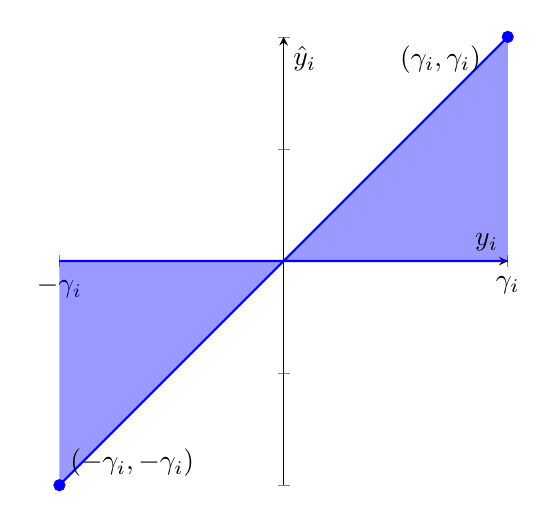
\begin{tikzpicture}
		\begin{axis}[
			xlabel={$y_i$},
			ylabel={$\hat{y}_i$},
			xmin=-2, xmax=2,
			ymin=-2, ymax=2,
			axis lines=center,
			samples=100, 
			unit vector ratio=1 1 1, scale=1, xtick   = {-2,2},
			xticklabels = {$-\gamma_i$,$\gamma_i$},
			yticklabels = {},
			]
			\addplot[blue, thick, fill=blue, fill opacity=0.4] {x} \closedcycle; 
			\addplot[blue, thick] {0}; 
			
			\addplot[only marks, mark=*, mark size=2pt, blue] coordinates {(-2,-2)};
			\node[label={above:$(-\gamma_i,-\gamma_i)$}] at (axis cs: -1.35, -2.1) {};
			
			\addplot[only marks, mark=*, mark size=2pt, blue] coordinates {(2,2)};
			\node[label={above:$(\gamma_i,\gamma_i)$}] at (axis cs: 1.4, 1.5) {};
		\end{axis}
	\end{tikzpicture}
	
   Based on above constraints, we can sketch this simplified model:
\begin{enumerate}
	\item For each input node, each output node, and each pre-activation and post-activation node in the hidden layers,  set one variable $y_i$. 
	\item Set constraints for input nodes.
	\item Set linear constraints . In this case, since the meaning of $y_i$ is $x_i-x'_i$, this constraints will not use the bias.
	\item Between pre- and post- activation nodes, set the MILP constraint described above.
\end{enumerate}
	
	The advantage of this simplified model is that it only contains the number of binary variables as MILP model for local robustness, hence the running speed of this is much faster comparing to the previous one. The cost is a loss of accuracy when the time is infinite. 
	
	However, in practice, with a reasonable timeout, this simplified model can usually obtain a better bound.
	
	\subsection{Strength of the simplified model}

	The second simplified model is more complex than the first.
	
	We can use the following extra constraints (besides 4 constraints about $\hat{x}_i'=\ReLU(x_i')$) to build this relation:
	
	
	\begin{align*}
		&\hat{y}_i \geq -\hat{x}'_i \hspace*{1ex} \wedge \hspace*{1ex} \hat{y}_i \leq -\hat{x}'_i+a\beta_i  \hspace*{1ex}\wedge\hspace*{1ex} x_i'+y_i \leq a\beta_i \hspace*{1ex}\wedge\hspace*{1ex}  x_i'+y_i \geq (1-a)\alpha_i \\
		&\hat{y}_i \geq -\hat{x}'_i+(x_i'+y_i) \hspace*{1ex}\wedge\hspace*{1ex} \hat{y}_i \leq -\hat{x}'_i+(x_i'+y_i) +(a-1)\alpha_i \\
	\end{align*} 
	
	
	Moreover, we can add two more natural constraints: $x_i'+y_i \geq \alpha_i \hspace*{1ex}\wedge\hspace*{1ex}  x_i'+y_i \leq \beta_i.$
	
	
	
	A more direct way to establish the constraints is as follows: \begin{align*}
		& y_i+x'_i \leq a\beta_i \quad\wedge \quad y_i+x'_i\geq (1-a)\alpha_i\\	
		& x_i' \leq a'\beta_i \quad\wedge \quad x_i'\geq (1-a')\alpha_i\\
		&\hat{y}_i \leq a\gamma_i \quad\wedge \quad	\hat{y}_i \geq -a'\gamma_i \\
		&	\hat{y}_i \leq y_i+(1-a)\gamma_i \quad\wedge \quad	\hat{y}_i \geq y_i - (1-a')\gamma_i \\
		&	\hat{y}_i \leq -x'_i+a\beta_i \quad\wedge \quad	\hat{y}_i \geq -x'_i+(1-a')\alpha_i \\
		&	\hat{y}_i \leq y_i+x'_i+(1-a)(-\alpha_i)\quad\wedge \quad	\hat{y}_i \geq y_i+x'_i+a'(-\beta_i) \\
	\end{align*}The following two plots show its shape:
	
	\iffalse
	\hspace*{-10ex}
	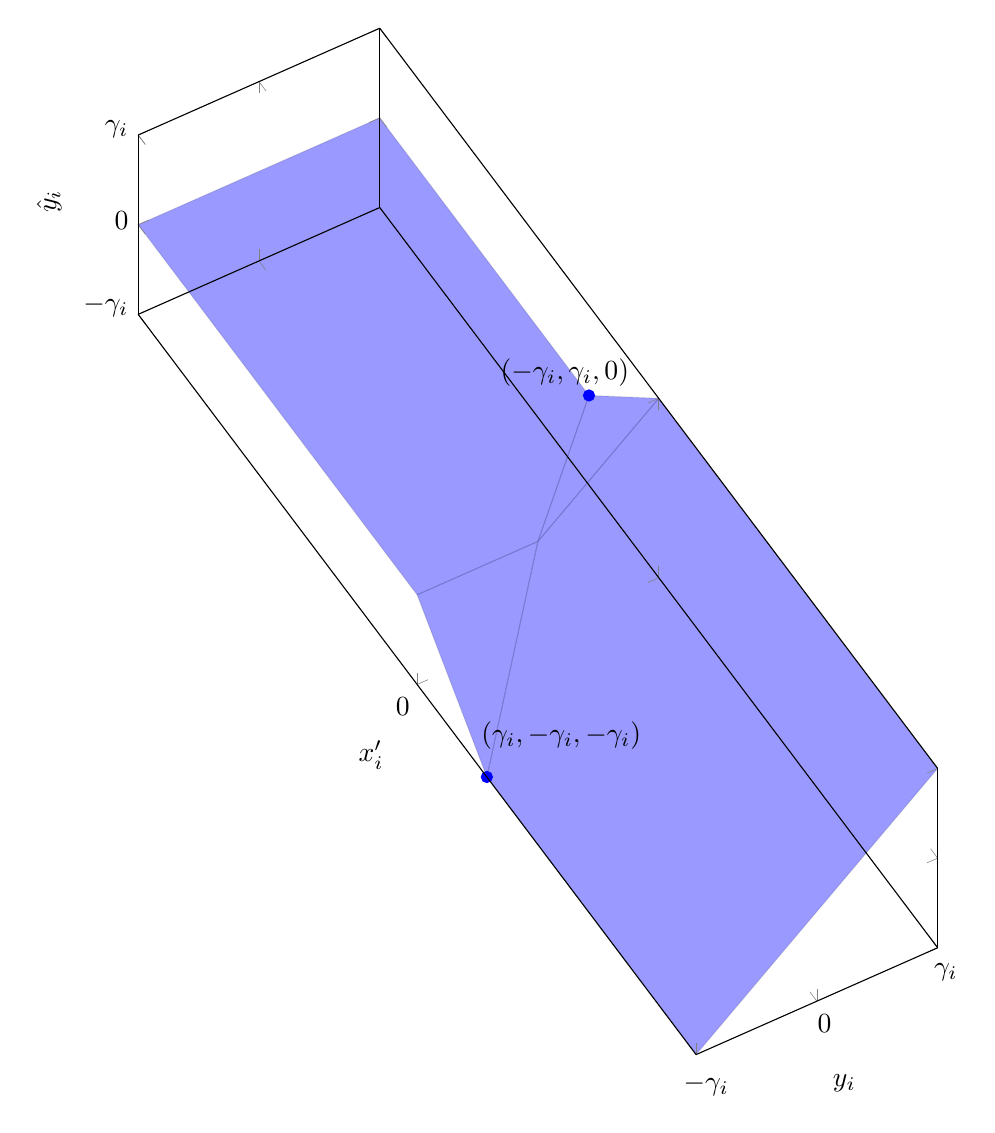
\begin{tikzpicture}
		\begin{axis}[	axis on top, xlabel = \(x'_i\),
			ylabel = {\(y_i\)}, zlabel = \(\hat{y}_i\),
			set layers=default,
			xmax = 4, xmin = -4,
			ymax = 1, ymin = -1,		
			zmax = 1, zmin = -1,
			unit vector ratio=1 1 1, scale=3,
			view={60}{50}, ytick   = {-1,0,1},
			yticklabels = {$-\gamma_i$,$0$,$\gamma_i$}, xtick = {0},
			xticklabels = {$0$}, ztick   = {-1,0,1},
			zticklabels = {$-\gamma_i$,$0$,$\gamma_i$},
			]
			\addplot3[fill=blue,opacity=0.1, fill opacity=0.4] 
			coordinates {
				(0,0,0) (-1,1,0) (-4,1,0) (-4,-1,0) (0,-1,0) (0,0,0)
			};
			
			\addplot3[fill=blue,opacity=0.1, fill opacity=0.4	] 
			coordinates { (0,0,0) (0,1,1) (4, 1, 1) (4, -1, -1) (1,-1,-1) (0,0,0)
			};
			
			\addplot3[fill=blue,opacity=0.1, fill opacity=0.4	] 
			coordinates { (0,0,0)  (-1,1,0) (0,1,1) (0,0,0)
			};
			
			\addplot3[fill=blue,opacity=0.1, fill opacity=0.4	] 
			coordinates { (0,0,0)  (0,-1,0) (1,-1,-1) (0,0,0)
			};
			
			\addplot3[only marks, mark=*, mark size=2pt, blue] coordinates {(1,-1,-1)};
			\node[label={$(\gamma_i,-\gamma_i, -\gamma_i)$}] at (axis cs: 1.2, -0.5 ,-1) {};
			
			\addplot3[only marks, mark=*, mark size=2pt, blue] coordinates {(-1,1,0)};
			\node[label={$(-\gamma_i,\gamma_i, 0)$}] at (axis cs: -1, 0.8 ,0) {};			
			
		\end{axis}
	\end{tikzpicture}
	\fi
	
	
	\hspace*{-15ex}
	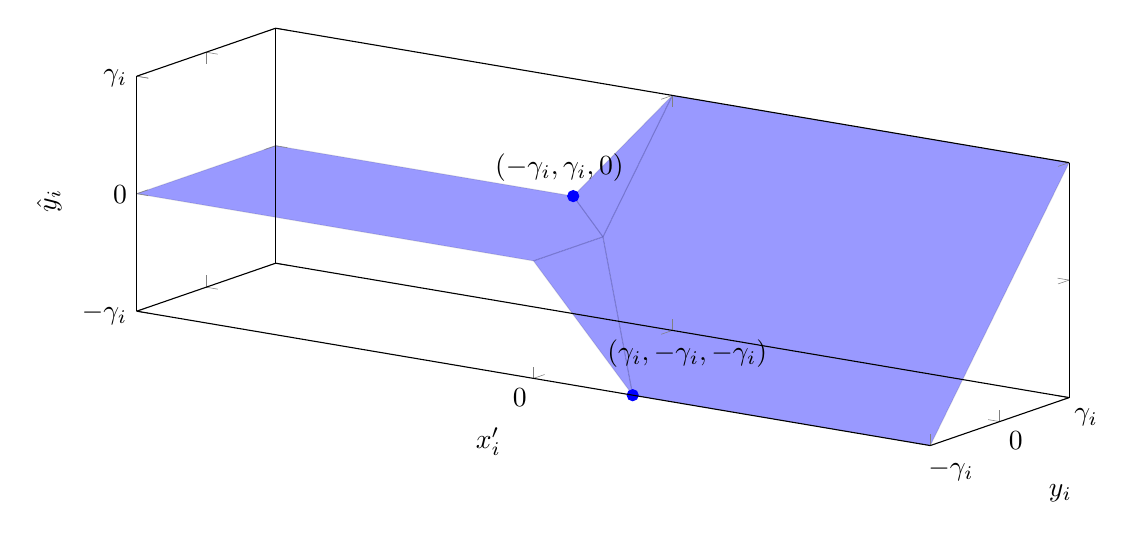
\begin{tikzpicture}
		\begin{axis}[	axis on top, xlabel = \(x'_i\),
			ylabel = {\(y_i\)}, zlabel = \(\hat{y}_i\),
			set layers=default,
			xmax = 4, xmin = -4,
			ymax = 1, ymin = -1,		
			zmax = 1, zmin = -1,
			unit vector ratio=1 1 1, scale=2.5,  ytick   = {-1,0,1},
			yticklabels = {$-\gamma_i$,$0$,$\gamma_i$}, xtick = {0},
			xticklabels = {$0$}, ztick   = {-1,0,1},
			zticklabels = {$-\gamma_i$,$0$,$\gamma_i$},
			view={35}{14},
			]
			\addplot3[ fill=blue,opacity=0.1, fill opacity=0.4] 
			coordinates {
				(0,0,0) (-1,1,0) (-4,1,0) (-4,-1,0) (0,-1,0) (0,0,0)
			};
			
			\addplot3[	fill=blue,opacity=0.1, fill opacity=0.4] 
			coordinates { (0,0,0) (0,1,1) (4, 1, 1) (4, -1, -1) (1,-1,-1) (0,0,0)
			};
			
			\addplot3[	fill=blue,opacity=0.1, fill opacity=0.4	] 
			coordinates { (0,0,0)  (-1,1,0) (0,1,1) (0,0,0)
			};
			
			\addplot3[	fill=blue,opacity=0.1, fill opacity=0.4	] 
			coordinates { (0,0,0)  (0,-1,0) (1,-1,-1) (0,0,0)
			};
			
			\addplot3[only marks, mark=*, mark size=2pt, blue] coordinates {(1,-1,-1)};
			\node[label={$(\gamma_i,-\gamma_i, -\gamma_i)$}] at (axis cs: 1.2, -0.5 ,-1) {};
			
			\addplot3[only marks, mark=*, mark size=2pt, blue] coordinates {(-1,1,0)};
			\node[label={$(-\gamma_i,\gamma_i, 0)$}] at (axis cs: -1, 0.8 ,0) {};			
			
		\end{axis}
	\end{tikzpicture}
	
	
	
	\section{Conclusion}
	
	TODO
	
	
	\bibliography{references}
	\bibliographystyle{plain}
	
	
	\bigskip
	
	\appendix
	
	
	
\end{document}


